\chapter*{Eclipse e Tomcat}
\label{apendice:eclipse_tomcat}

Neste Apêndice serão apresentados os passos necessários para a instalação e configuração do Tomcat e do Eclipse (IDE de desenvolvimento utilizado neste trabalho).

\section*{Eclipse}

Para utilizar a IDE de desenvolvimento Eclipse, é necessário fazer o download dele por meio da \textit{url} https://eclipse.org/downloads/. Ao acessar esta \textit{url} a página de \textit{download} será apresentada ao usuário conforme a Figura~\ref{fig:ap2:pagina_download_eclipse}.

\captionsetup[figure]{list=no}
\begin{figure}[h!]
	\centerline{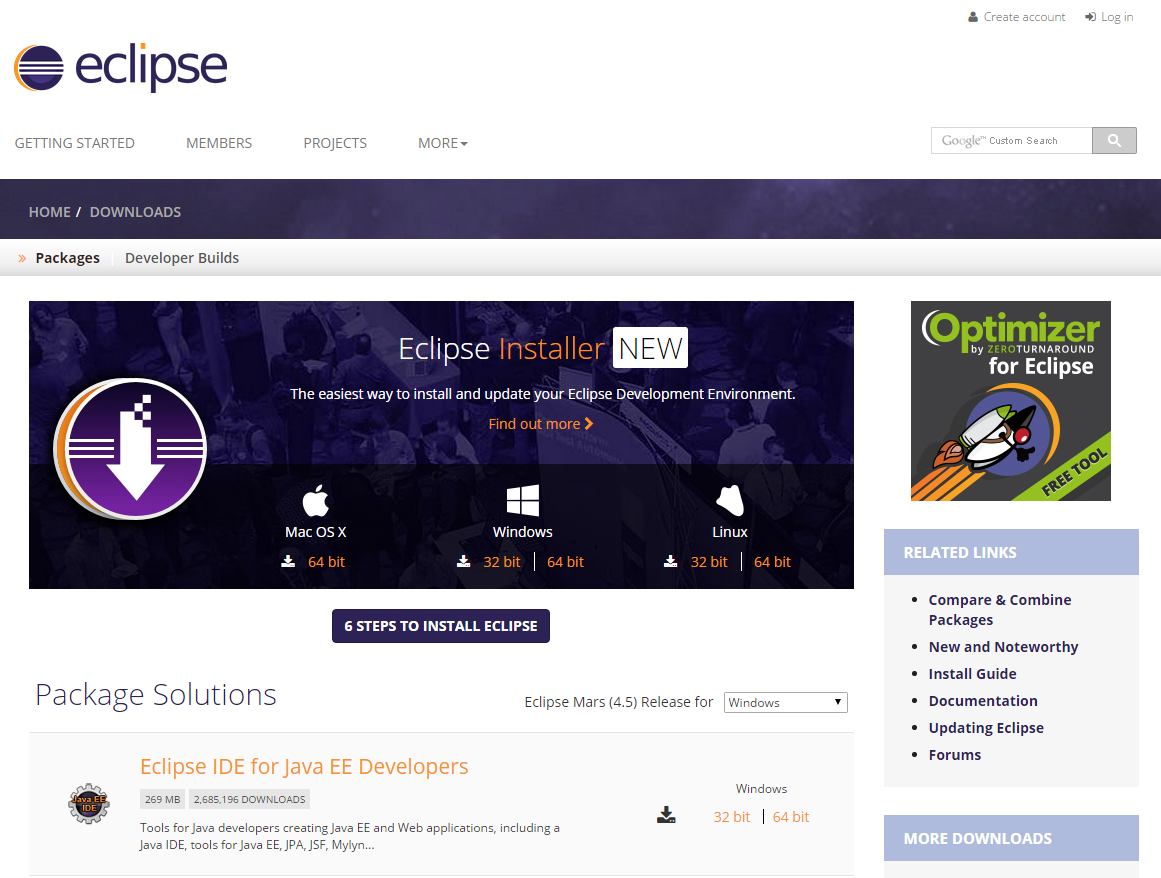
\includegraphics[scale=0.4]{./imagens/apendices/pagina-download-eclipse.png}}
	\caption[Página de \textit{download} do Eclipse.]
	{Página de \textit{download} do Eclipse. \textbf{Fonte:} Elaborado pelos autores.}
	\label{fig:ap2:pagina_download_eclipse}
\end{figure}

Nesta página o usuário deve selecionar qual a versão do sistema operacional ele utiliza para realizar o \textit{download} da versão correta.

Após realizado o download, o usuário deve descompactar o arquivo obtido e armazená-lo na pasta que desejar. Para iniciar o eclipse o usuário deve executar o arquivo eclipse.bat para sistemas operacionais Windows ou eclipse.sh para sistemas baseados em Unix como o Linux ou o OS X.

Após a executação deste arquivo o Eclipse, solicitará o diretório para criação do diretório de trabalho que ele irá utilizar, nesse momento o usuário deve informar um diretório válido. A Figura~\ref{fig:ap2:eclipse_selecionar_workspace} apresenta esta configuração.

\captionsetup[figure]{list=no}
\begin{figure}[h!]
	\centerline{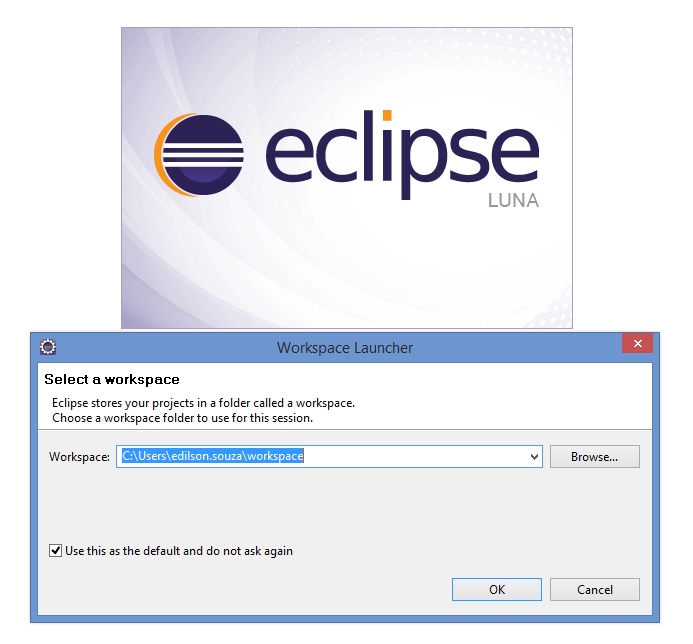
\includegraphics[scale=0.5]{./imagens/apendices/eclipse-selecionar-workspace.png}}
	\caption[Tela de definição de diretório de trabalho do Eclipse.]
	{Tela de definição de diretório de trabalho do Eclipse. \textbf{Fonte:} Elaborado pelos autores.}
	\label{fig:ap2:eclipse_selecionar_workspace}
\end{figure}

Após realizar os procedimentos descritos nesta seção, a tela inicial do eclipse será apresentada ao usuário, que, nesse instante estará apto a utilizá-lo e realizar as devidas configurações.

\section*{Tomcat}

Para utilizar o Tomcat foi necessario fazer o \textit{download} dele por meio da \textit{url} https://tomcat.apache.org, após acessá-la, selecione a versão que deseja e clique sob ela. A Figura~\ref{fig:ap2:pagina_inicial_apache_tomcat}.

\newpage
\captionsetup[figure]{list=no}
\begin{figure}[h!]
	\centerline{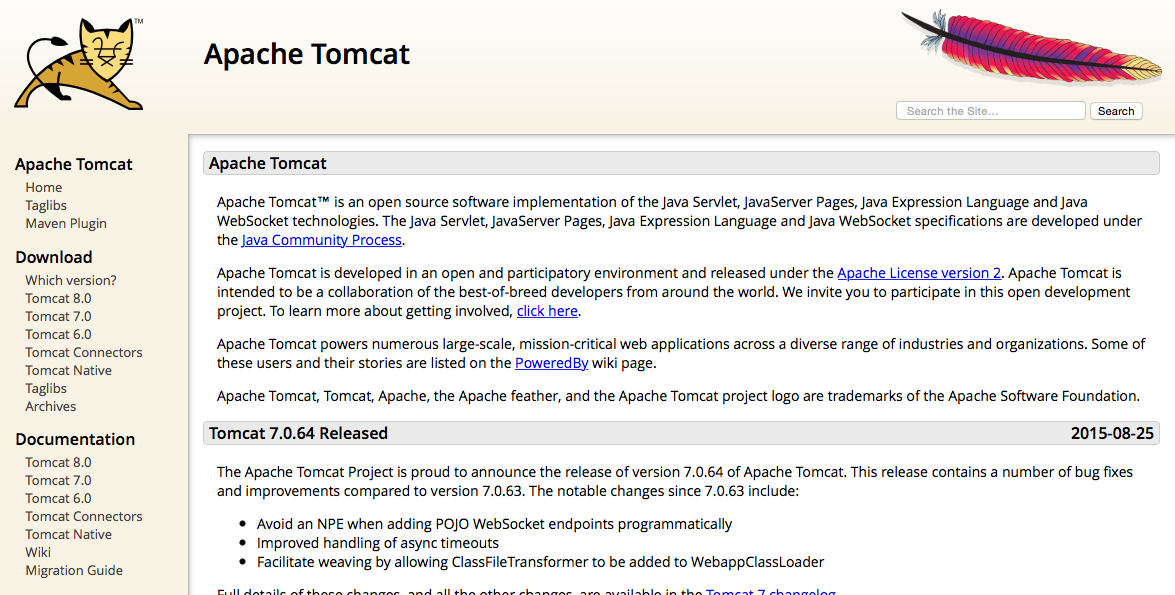
\includegraphics[scale=0.35]{./imagens/apendices/pagina-inicial-apache-tomcat.png}}
	\caption[Página inicial do Tomcat.]
	{Página inicial do Tomcat. \textbf{Fonte:} Elaborado pelos autores.}
	\label{fig:ap2:pagina_inicial_apache_tomcat}
\end{figure}

Após a seleção da versão do Tomcat a página específica da versão selecionada será apresentada ao usuário conforme a Figura~\ref{fig:ap2:pagina_download_apache_tomcat}. Clique na opção desejada para realizar o \textit{download}. Neste trabalho foi utilizada a versão compactada do \textit{Core}.

\captionsetup[figure]{list=no}
\begin{figure}[h!]
	\centerline{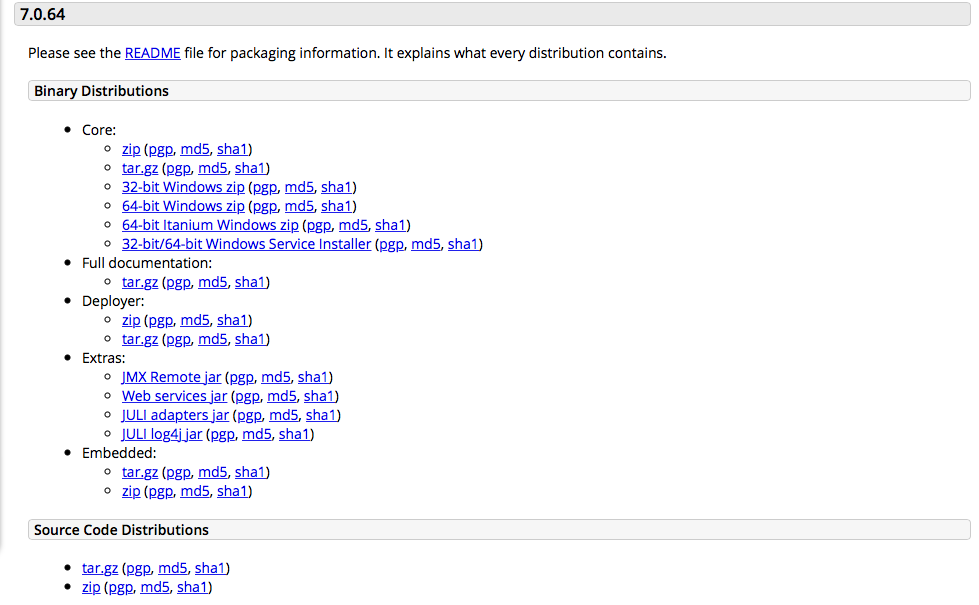
\includegraphics[scale=0.4]{./imagens/apendices/pagina-download-tomcat-7.png}}
	\caption[Página para \textit{download} do Tomcat.]
	{Página para \textit{download} do Tomcat. \textbf{Fonte:} Elaborado pelos autores.}
	\label{fig:ap2:pagina_download_apache_tomcat}
\end{figure}

Após o processo de \textit{dowload} concluído, deve-se descompactar o arquivo obtido em um diretório.

\subsection*{Configuração do Tomcat}

Para utilizar o Tomcat em conjunto com o Eclipse, foi necessário realizar algumas configurações que serão apresentadas a seguir.

Com o Eclipse sendo executado, abra a perspectiva \textit{Server} como demonstra a Figura~\ref{fig:ap2:perspectiva_server_no_server_eclipse} e clique no \textit{link} apresentado.

\captionsetup[figure]{list=no}
\begin{figure}[h!]
	\centerline{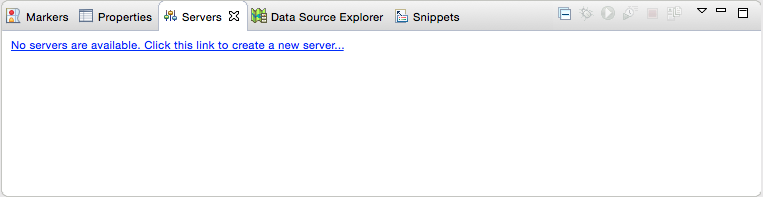
\includegraphics[scale=0.5]{./imagens/apendices/perspectiva-server-sem-servidor.png}}
	\caption[Perspectiva \textit{Server} do Eclipse.]
	{Perspectiva \textit{Server} do Eclipse. \textbf{Fonte:} Elaborado pelos autores.}
	\label{fig:ap2:perspectiva_server_no_server_eclipse}
\end{figure}

Uma nova tela será apresentada solicitando ao usuário que selecione a versão do servidor que deseja adicionar como mostra a Figura~\ref{fig:ap2:selecioanr_versao_server_adicionar_eclipse}, após esta definição clique no botão \textit{"Next"}.

\captionsetup[figure]{list=no}
\begin{figure}[h!]
	\centerline{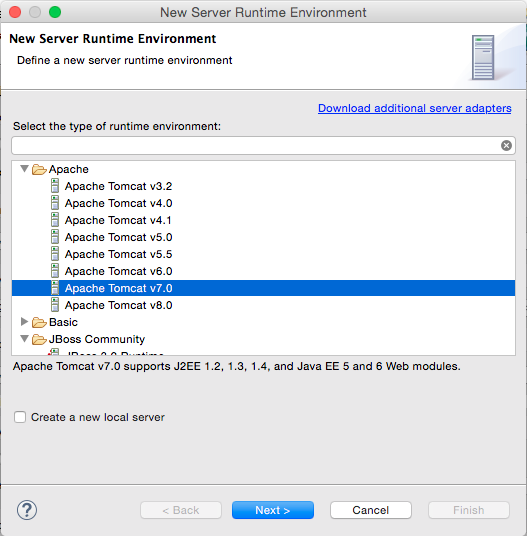
\includegraphics[scale=0.4]{./imagens/apendices/criar-configuracao-tomcat-no-eclipse.png}}
	\caption[Definir a versão do novo servidor no Eclipse.]
	{Definir a versão do novo servidor no Eclipse. \textbf{Fonte:} Elaborado pelos autores.}
	\label{fig:ap2:selecioanr_versao_server_adicionar_eclipse}
\end{figure}

Após selecionar a versão do Tomcat, deve-se informar na próxima tela, como apresenta a Figura~\ref{fig:ap2:definir_diretorio_tomcat_no_eclipse}, as informações a respeito do diretório cujo Tomcat foi extraído e, sob qual versão do Java ele será executado, com essas informações definidas clique no botão \textit{"Finish"}.

\newpage
\captionsetup[figure]{list=no}
\begin{figure}[h!]
	\centerline{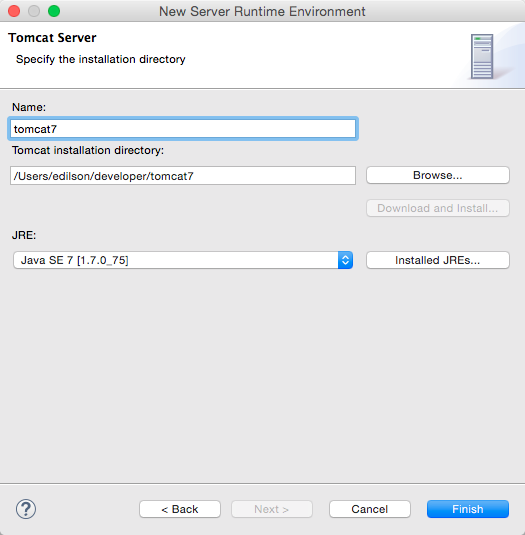
\includegraphics[scale=0.4]{./imagens/apendices/definir-pasta-home-tomcat.png}}
	\caption[Definir as configurações do Tomcat no Eclipse.]
	{Definir as configurações do Tomcat no Eclipse. \textbf{Fonte:} Elaborado pelos autores.}
	\label{fig:ap2:definir_diretorio_tomcat_no_eclipse}
\end{figure}

Após realizado todos os procedimentos descritos neste Apêndice, a IDE Eclipse em conjunto com o Tomcat estarão prontos para serem utilizados.
